% !TEX TS-program = LuaLaTeX
\documentclass[11pt,compress,xcolor=x11names,UTF8]{beamer}
\usetheme{Boadilla}
\usecolortheme{seahorse}
\useinnertheme[shadow]{rounded}  
\useoutertheme[subsection=false]{smoothbars}
\usecolortheme{spruce}
\usecolortheme[named=SpringGreen4]{structure}
\usefonttheme{structurebold}
\useinnertheme{circles}
\usecolortheme{rose}
\usepackage{pifont}
\usepackage{academicons}
\usepackage{fontawesome}
\usepackage{iitem}
%\usepackage{graphicx}
%\usepackage{tabular}
\setbeamertemplate{itemize item}{\ding{108}}
\setbeamertemplate{itemize subitem}{\ding{109}}
\setbeamertemplate{navigation symbols}{}
\setbeamercovered{transparent}  
\renewcommand\appendixname{附录}
\renewcommand\abstractname{摘要}
\graphicspath{{figure/}} % 图片路径
\usepackage{calligra} % Thank you
\usepackage{ctex} % 加入中文
%\setCJKsansfont{Noto Sans CJK SC}
\setsansfont{Lato} % Lato Roboto Fira Sans
\usepackage{makecell}
\newcommand{\tabincell}[2]{\begin{tabular}{@{}#1@{}}#2\end{tabular}}
\usepackage{url}					
\usepackage{natbib} % 参考文献
%\title[Spatial Generalized Linear Mixed Models]{Spatial Generalized Linear Mixed Models with Application to Prevalence Mapping}
\title{Container PMT Testing Data in ROOT format}
%\subtitle{奖助金申请答辩}
\author[Rong. Zhao]{Email:zhaor25@mail2.sysu.edu.cn \and  } % \\ 专业:统计学 \\ 方向:数据分析与统计计算
\institute[Sun Yat-Sen University]{School of Physics\and } % 理学院\\
\date[\today]{
\includegraphics[width=.5\textwidth]{logo}}

\begin{document}

\maketitle

%\begin{frame}{Outline}
%\tableofcontents
%\end{frame}

\section{Introduction}

%\subsection{研究意义}

%\begin{frame}{motivation}
%%\textsf{例} \textbf{例}  \textit{例} 
%% \texttt{例}  % 调出仿宋字体了
%	Due to complex of PMT testing procedure and upgrades of hardware and software, the raw data of PMT testing is not user-frinedly.
%\vspace{.5cm}
%
%	\alert{It is a good choice to produce a uniform structure to re-organize and store the raw data.}
%\begin{table}[]  
%\caption{PMT typical performance}  
%\resizebox{.8\textwidth}{!}{%
%\begin{tabular*}{.98\textwidth}{l|cccc}
%%\toprule  
%\hline  
%\hline  
%Performance & PDE &DCR & TTS& uniformity \\  
%\hline  
%HAMAMATSU &  lower\% & 20 kHz& 3ns& worse \\  
%NNVT  & higher\% & 40kHz & 7ns& better \\  
%\hline  
%\end{tabular*}  
%%}
%\end{table} 
%\begin{figure}
%\centering
%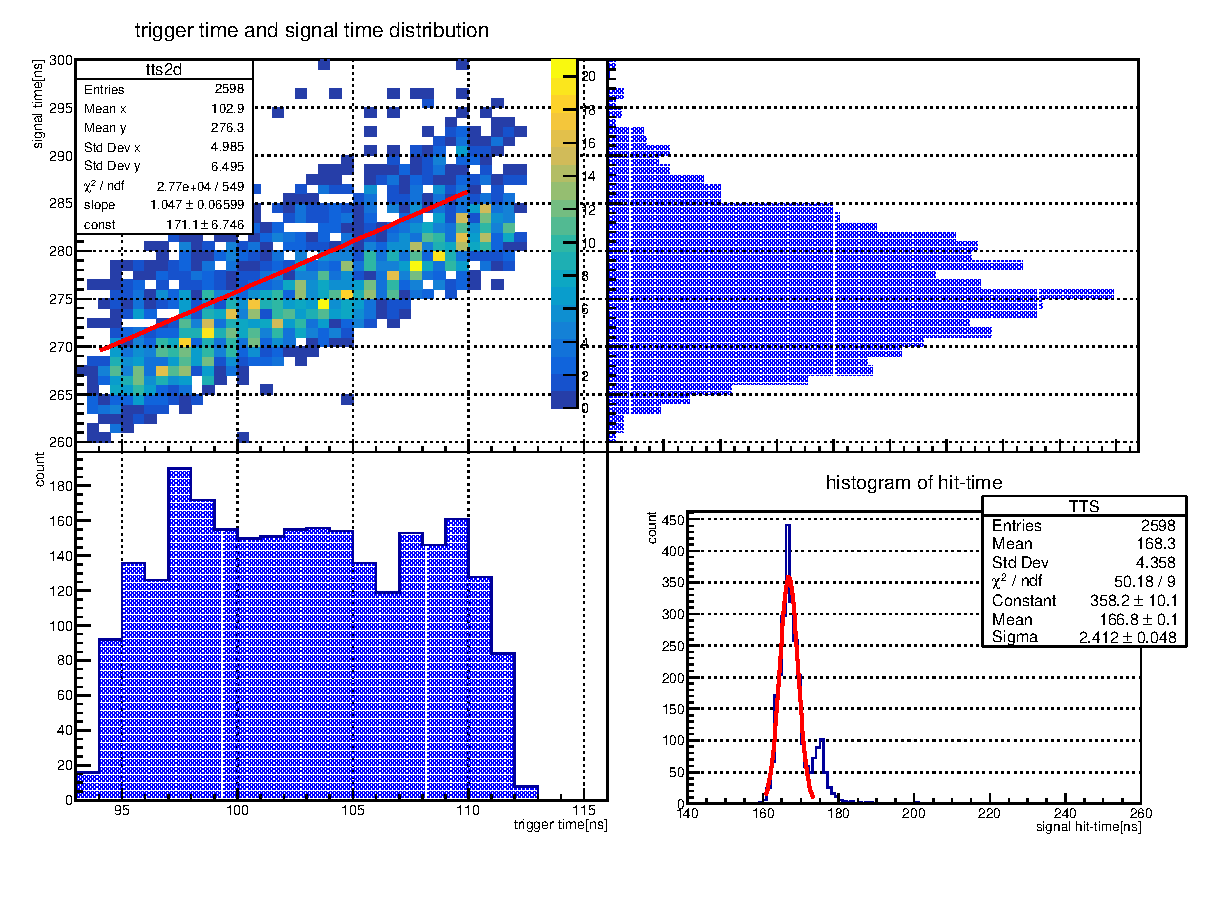
\includegraphics[width=0.78\textwidth]{typical_hittime} % 单图
%\end{figure}
%\end{frame}
%%%%%%%%%%%%%%%%%%%%%%%%%%%%%%%%%%%%%%%%%%%
\begin{frame}{ introduction }
	\begin{enumerate}
		\item Onsite server:login.pmt.ihep.ac.cn  \footnote{https://juno.ihep.ac.cn/mediawiki/index.php/Onsite\_computing/IT}
		\item raw testing data path: /pmtfs/disk01/container\_data/Meassurements\_DAQ
		\item output ROOT file path: /pmtfs/disk01/container\_data/rawdata 
		\item file size: about 500Mb for one PMT each test.
		\item name rule: container#+drawer#+SN
	\end{enumerate}
\end{frame}
%%%%%%%%%%%%%%%%%%%%%%%%%%%%%%%%%%%%%%%%%%%
\begin{frame}{inside one ROOT file}
One can get 13 trees and one TObject "Pmtdata" from the ROOT file
\begin{figure}
\centering
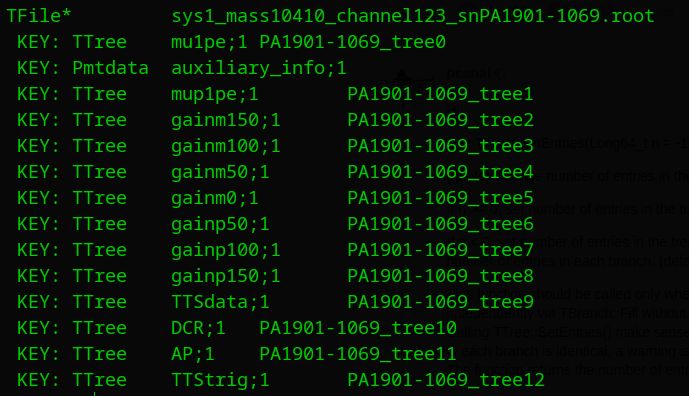
\includegraphics[width=0.78\textwidth]{rootfile} % 单图
\end{figure}
\end{frame}
\section{calibration of drawer}
%%%%%%%%%%%%%%%%%%%%%%%%%%%%%%%%%%%%%%%%%%%
\begin{frame}{TObject:Pmtdata}
The custom class "Pmtdta" is inherited from TObject, and it store the auxiliary information of one pmttest such as: SN,test-date,HV,base .etc.
\begin{figure}
\centering
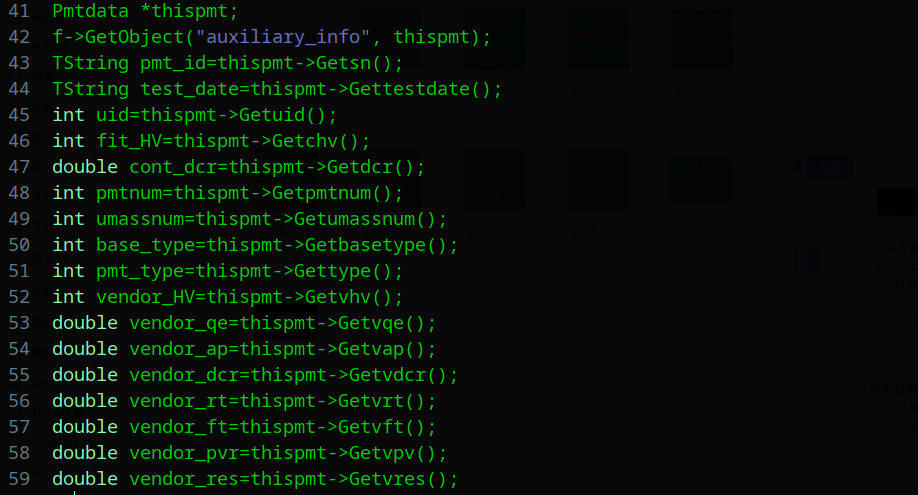
\includegraphics[width=0.88\textwidth]{pmtdataclass} % 单图
\end{figure}
\end{frame}
%%%%%%%%%%%%%%%%%%%%%%%%%%%%%%%%%%%%%%%%%%%
%~~!!!!!!!!!!!!!!!!!!put two figures to illustrate!!!!!
\begin{frame}{waveform data}
There are 11 trees for the storage of testing waveform:
	\begin{itemize}
\item mu1pe$\rightarrow$ with the LED light intensity @ $\mu \simeq 1$.
\item mup1pe$\rightarrow$   with the LED light intensity @ $\mu \simeq 0.1$.
\item gain...$\rightarrow$ with the LED light intensity @ $\mu \simeq 0.1$ and HV=vendor HV+\{-150V,-100V,-50V,0V,50V,100V,150V\}. 
\item TTSdata$\rightarrow$ waveforms for TTS test.
\item TTStrig$\rightarrow$ waveforms for the trig signals of TTS test.
	\end{itemize}
Each waveform is a "TVector" with length 500, and the value is in mV unit.

	\vspace{.5cm}
Also, the "DCR" tree is for dark count rate data and "AP" tree is for afterpulse data. The values are accumulated DCRs with 1s step. 
\end{frame}
%%%%%%%%%%%%%%%%%%%%%%%%%%%%%%%%%%%%%%%%%%%
\begin{frame}{simple test for the ROOT file}
read the TTS and mu1pe waveform from ROOT :
\begin{figure}
\centering
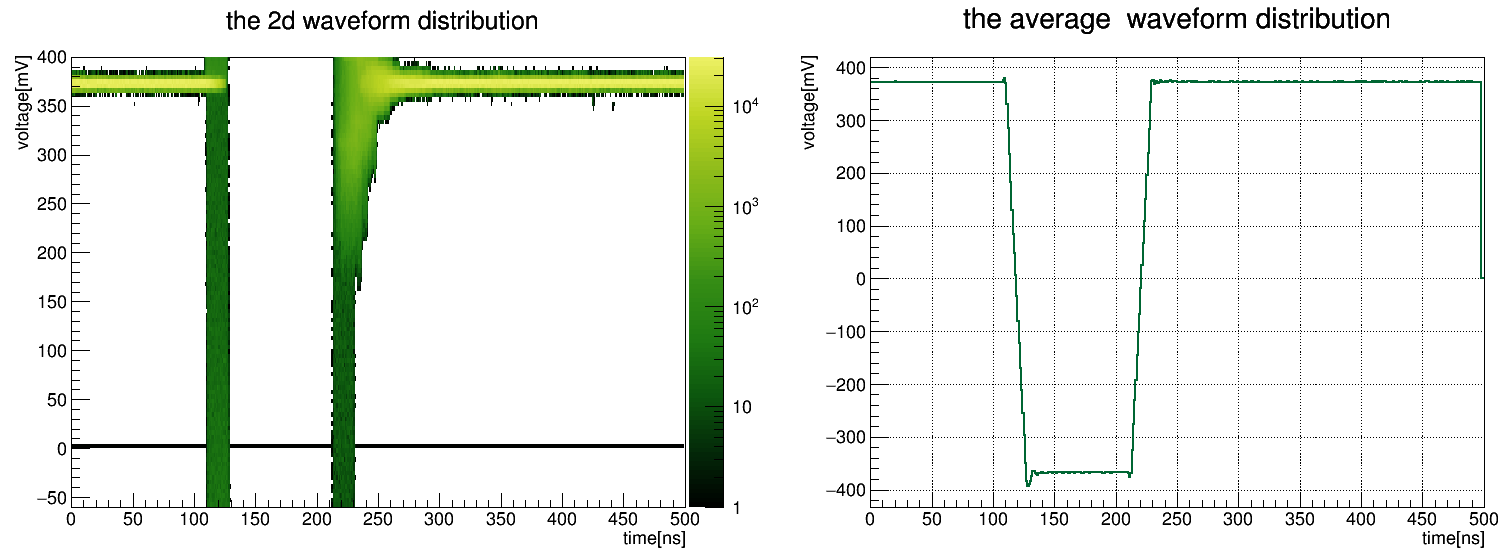
\includegraphics[width=0.68\textwidth]{ttswave} % 单图
\end{figure}
\begin{figure}
\centering
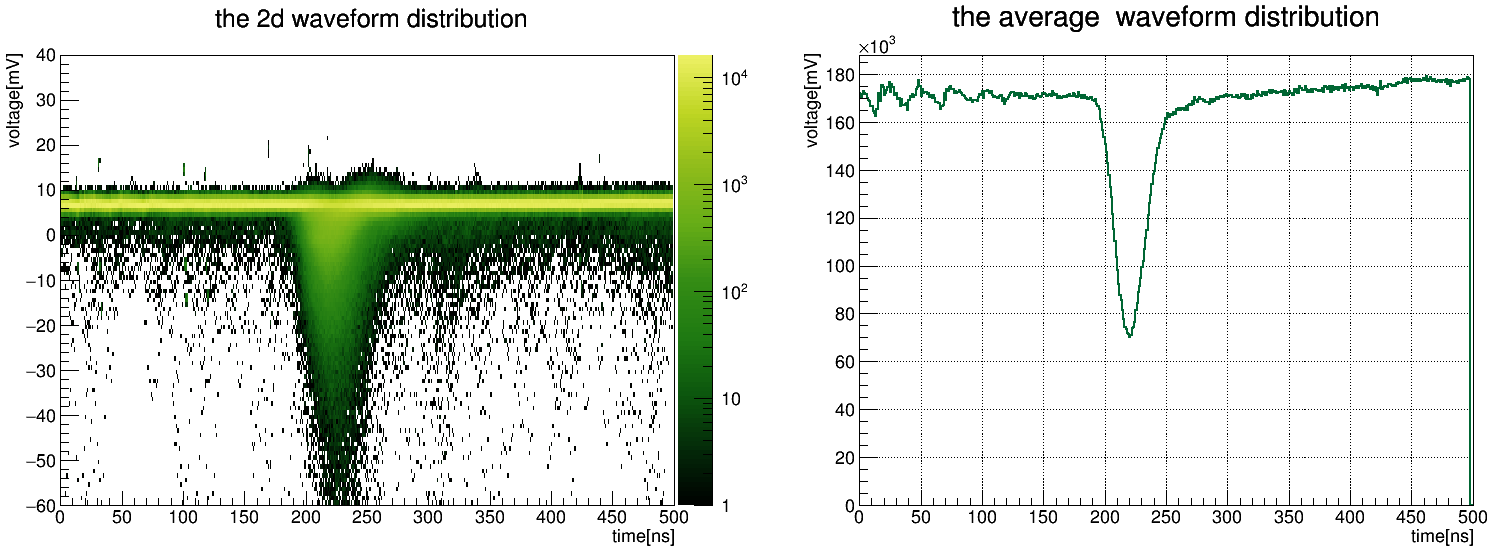
\includegraphics[width=0.68\textwidth]{mu1pe} % 单图
\end{figure}
\end{frame}
%%%%%%%%%%%%%%%%%%%%%%%%%%%%%%%%%%%%%%%%%%%

%%%%%%%%%%%%%%%%%%%%%%%%%%%%%%%%%%%%%%%%%%%%%%%%%%%%%%%%%%%%%%%%%%%%
%\section{PMT orientation}
%%%%%%%%%%%%%%%%%%%%%%%%%%%%%%%%%%%%%%%%%%%%%%%%%%%%%%%%%%%%%%%%%%%%
\begin{frame}{HAMAMATSU PMTs}
the PDE uniformity of HAMAMATSU PMTs are not so good
\hrule{\textwidth}
we can artificially correct the PDE if these PMTs have fixed orientation and we can extract the light incident angle using reconstraction information.
\end{frame}
%%%%%%%%%%%%%%%%%%%%%%%%%%%%%%%%%%%%%%%%%%%%%%%%%%%%%%%%%%%%%%%


\begin{frame}
\centering {\zihao{0} \color{red} \calligra{Back-Up}}

\end{frame}
%%%%%%%%%%%%%%%%%%%%%%%%%%%%%%%%%%%%%%%%%%%
\begin{frame}{load the Pmtdata class}
	to use the shared library:\\
CINT mode: gSystem->Load("/home/pmthome/zhaor/zhaorong/cont\_v1/pmttest\_cc.so");\\
in script: R\_\_LOAD\_LIBRARY(/home/pmthome/zhaor/zhaorong/cont\_v1/\\
	pmttest\_cc.so);
\end{frame}


%\begin{frame}[allowframebreaks]
%\frametitle{References}
%\scriptsize
%\bibliographystyle{authordate1}
%\bibliography{R-GLMM-pkgs}
%\end{frame}

\appendix

\section*{附录}


\end{document} 


